% This file is part of Bachelorarbeit

% Bachelorarbeit is free software: you can redistribute it and/or modify
% it under the terms of the GNU General Public License version 3 as published by
% the Free Software Foundation.

% Bachelorarbeit is distributed in the hope that it will be useful,
% but WITHOUT ANY WARRANTY; without even the implied warranty of
% MERCHANTABILITY or FITNESS FOR A PARTICULAR PURPOSE.  See the
% GNU General Public License for more details.

% You should have received a copy of the GNU General Public License
% along with Foobar. If not, see <http://www.gnu.org/licenses/>.

\section{Vorgehensweise}


\subsection{Portierung von libipsec auf Windows}
Die Portierung von libipsec auf Windows, sodass sie dort lauffähig ist, ist das Ziel
der Bachelorarbeit. Die zu portierenden Teile des Programmcodes betreffen nur
die Codesegmente, die Plattformspezifische \acp{API} oder \acp{ABI} verwenden,
also primär alles um Dateiein- und ausgabe, sowie das verwalten von TUN-Geräten.
Unter Unix und Linux werden hier \acp{FD} verwendet. Unter Windows werden stattdessen
Handles genutzt, welche einen anderen Dateityp darstellen. Des weiteren unterscheidet
sich die Methode zum Multiplexen von Lese-Aufrufen einer Liste von Dateien stark.
Unter Unix und Linux wird hierfür poll() genutzt, unter Windows geschieht das jedoch
Event-basiert mit WaitForMultipleObjects().
Explizite Beispiele hierfür sind im Abschnitt über die Portierung von libipsec sichtbar.
Bei der Portierung wurde für das verwalten von Speicherabschnitten 
primär alloca() genutzt, statt malloc() und seine Unterarten. Der Unterschied hierbei ist die
Speicherdauer. Mit alloca() allokierter Speicher ist nur bis zum Verlassen der Funktion gültig
und wird automatisch freigegeben. Mit malloc() allokierter Speicher muss manuell freigegeben werden.
alloca() ist ein Feature, welches nicht standardisiert ist.
Daher lässt sich strongSwan nicht mit allen C-Bibliotheken übersetzen.
Auf der Wiki-Seite über den Windows-Port wird erwähnt, dass nur die Kompilierung
mittels MinGW-W64 unterstützt wird.


\subsection{Bestehende Implementierung}
Die bestehende Implementierung umfasst die eigentliche Bibliothek, eine Implementierung
eines Kernel-Interface zwischen libipsec und charon, sowie Code in libstrongswan
um TUN-Geräte zu öffnen. Martin Willi hat 2014 bereits die gesamte Portierungsarbeit
für version 5.2.0 von strongSwan gemacht. Der Port unterstützt Windows 7 / server 2008 R2
und neuer.

\subsection{Unterstützte Kryptographie}
Die unterstützte Kryptographie ist notwendigerweise von den deklarierten Identifikatoren
für IKE beschränkt. strongSwan unterstützt mehr Verschlüsselungsalgorithmen als
in den \acp{RFC} deklariert wurde. Aus diesem Grund nutzt strongSwan Identifikatoren
teilweise aus dem privaten Bereich, wenn die Identifikatoren für den eingesetzten Algorithmus
nicht standardisiert sind.

strongSwan unterstützt eine große Anzahl von Algorithmen im Vergleich zu anderen Implementierungen,
wie in den Tabellen in \autoref{sec:appendix} dagelegt wird. Wenn libipsec genutzt wird,
so können alle Algorithmen, die im Userspace implementiert sind, für die Absicherung
von Verkehr genutzt werden.

\subsection{Portierung}
\subsubsection{header}
Die Bibliotheken und Plugins um libipsec nutzen diverse Datenstrukturen und Konstanten,
die in C-Header-Dateien von Linux definiert sind. Diese sind unter Windows nicht verfügbar.
Aus diesem Grund wurde eine Kopie der relevanten Definitionen in den Quellcode kopiert
und fehlende Teile ergänz.
Spezifisch wurde aus dem Quellcode von GLIBC die Definition eines \ac{IP}-Headers kopiert
und die fehlenden Protokollkonstanten per Hand ergänzt.

Folgend ist die Headerdatei

\begin{lstlisting}[caption=Header für libipsec]
/* Copyright (C) 1991-2016 Free Software Foundation, Inc.
   This file is part of the GNU C Library.

   The GNU C Library is free software; you can redistribute it and/or
   modify it under the terms of the GNU Lesser General Public
   License as published by the Free Software Foundation; either
   version 2.1 of the License, or (at your option) any later version.

   The GNU C Library is distributed in the hope that it will be useful,
   but WITHOUT ANY WARRANTY; without even the implied warranty of
   MERCHANTABILITY or FITNESS FOR A PARTICULAR PURPOSE.  See the GNU
   Lesser General Public License for more details.

   You should have received a copy of the GNU Lesser General Public
   License along with the GNU C Library; if not, see
   <http://www.gnu.org/licenses/>.  */

*/

/*
 * Copyright (c) 1982, 1986, 1993
 *      The Regents of the University of California.  All rights reserved.
 *
 * Redistribution and use in source and binary forms, with or without
 * modification, are permitted provided that the following conditions
 * are met:
 * 1. Redistributions of source code must retain the above copyright
 *    notice, this list of conditions and the following disclaimer.
 * 2. Redistributions in binary form must reproduce the above copyright
 *    notice, this list of conditions and the following disclaimer in the
 *    documentation and/or other materials provided with the distribution.
 * 4. Neither the name of the University nor the names of its contributors
 *    may be used to endorse or promote products derived from this software
 *    without specific prior written permission.
 *
 * THIS SOFTWARE IS PROVIDED BY THE REGENTS AND CONTRIBUTORS ``AS IS'' AND
 * ANY EXPRESS OR IMPLIED WARRANTIES, INCLUDING, BUT NOT LIMITED TO, THE
 * IMPLIED WARRANTIES OF MERCHANTABILITY AND FITNESS FOR A PARTICULAR PURPOSE
 * ARE DISCLAIMED.  IN NO EVENT SHALL THE REGENTS OR CONTRIBUTORS BE LIABLE
 * FOR ANY DIRECT, INDIRECT, INCIDENTAL, SPECIAL, EXEMPLARY, OR CONSEQUENTIAL
 * DAMAGES (INCLUDING, BUT NOT LIMITED TO, PROCUREMENT OF SUBSTITUTE GOODS
 * OR SERVICES; LOSS OF USE, DATA, OR PROFITS; OR BUSINESS INTERRUPTION)
 * HOWEVER CAUSED AND ON ANY THEORY OF LIABILITY, WHETHER IN CONTRACT, STRICT
 * LIABILITY, OR TORT (INCLUDING NEGLIGENCE OR OTHERWISE) ARISING IN ANY WAY
 * OUT OF THE USE OF THIS SOFTWARE, EVEN IF ADVISED OF THE POSSIBILITY OF
 * SUCH DAMAGE.
 *
 *      @(#)ip.h        8.1 (Berkeley) 6/10/93
 */

/*
 * Details about licensing:
 * The definition of the IP header is from the headers of GLIBC, that come with Arch Linux
 * It is subject to the license headers of GLIBC and Berkeley
 * The IP protocol identifier constants are manually determined from /etc/protocols
 * and hand written out.  They are subject to the GPLv2.
 */

#ifndef WINDOWS_32_PROTOCOL_HEADERS
#define WINDOWS_32_PROTOCOL_HEADERS

/*
 * Structure of an internet header, naked of options.
 */
struct ip
  {
#if __BYTE_ORDER == __LITTLE_ENDIAN
    unsigned int ip_hl:4;               /* header length */
    unsigned int ip_v:4;                /* version */
#endif
    uint8_t ip_tos;                    /* type of service */
    u_short ip_len;                     /* total length */
    u_short ip_id;                      /* identification */
    u_short ip_off;                     /* fragment offset field */
#define IP_RF 0x8000                    /* reserved fragment flag */
#define IP_DF 0x4000                    /* dont fragment flag */
#define IP_MF 0x2000                    /* more fragments flag */
#define IP_OFFMASK 0x1fff               /* mask for fragmenting bits */
    uint8_t ip_ttl;                    /* time to live */
    uint8_t ip_p;                      /* protocol */
    u_short ip_sum;                     /* checksum */
    struct in_addr ip_src, ip_dst;      /* source and dest address */
  };

# 
#define IPPROTO_IPIP 4
#define IPPROTO_IPv6 41
#define IPPROTO_NONE 59

#endif /* WINDOWS_32_PROTOCOL_HEADERS */
\end{lstlisting}

\subsubsection{libipsec}
libipsec implementiert die Verarbeitung von Paketen, das Erzwingen der \acp{SP},
das Verwalten der \acp{SP}, \acp{SA}, Routen und der TUN-Geräte.
Die hierbei relevanten Dateien sind unter /src/libipsec/ zu finden.

Standardmäßig installiert strongSwan die IP-Adressen die per Config-Mode
oder \ac{CP} empfangen wird auf dem ausgehenden Interface (Linux, Kernelspace processing),
was für die Kommunikation mit dem Peer genutzt wird,
oder auf dem loopback-Adapter (Windows).
Um die IP-Adresse für TUN-Geräte korrekt zu setzen, nutzt libipsec den Parameter
"charon.install\_virtual\_ip\_on" von strongswan.conf, der während der Initialisierung
des Plugins gesetzt wird.
% route installation
% queues
% processing
% event driven
% job
\subsubsection{kernel-libipsec}
Die hier zu portierenden Bestandteile waren ausschließlich Codeteile, die
sich mit der Dateiein- und ausgabe beschäftigten.

Die primäre Aufgabe hier war die Installation der Routen in ''kernel\_libipsec\_ipsec.c''
für Windows anzupassen, da hier ein Gateway verwendet wird auf einem TAP-Gerät
statt ein echtes TUN-Gerät, sowie die Anpassung des Codes für die Ein- und Ausgabe 
und einige Methoden in
''kernel\_libipsec\_router.c'', da das Multiplexen der Handles, sowie die Benachrichtigung
von anderen Threads auf Windows anders abläuft als auf Linux und Unix.

Für das Multiplexen der Eingabe stehen unter Windows zwei Verfahren zur Verfügung:
\begin{itemize}
\item WaitForMultipleObjects
\item IOCompletionPorts
\end{itemize}

WaitForMultipleObjects\footcite[][]{_waitformultipleobjects_2016} funktioniert mit einem Array aus Handles. In der Struktur des Handles
ist das event-Attribut auf ein einzgartiges Event gesetzt, welches genutzt wird um
das Handle zu finden, dessen Lesevorgang abgeschlossen oder abgebrochen wurde.
Nach dem Kopieren des Handles in das Array und dem Setzen des Events wird ein asynchroner
Lesevorgang gestartet. Wenn er sofort beendet wurde, wird das entsprechende Event gesetzt.
Dadurch beendet der Aufruf von WaitForMultipleObjects() nach dem aufruf direkt, falls
ein Lesevorgang schon zuvor erfolgreich war und der Programmcode wird etwas kürzer.
% Mehr Erläuterung benötigt

IOCompletionPorts\footcite[][]{_createiocompletionport_2016} funktionieren, indem man einen IOCompletionPort mit CreateIoCompletionPort()
anlegt und Handles mit ihm asoziiert. Bei der Asoziierung wird ein einzigartiger Schlüssel
übergeben, der bei der Signalisierung wieder zurückgegeben wird um das Handle identifizieren zu können.
Der CompletionPort kann erst nach dem Schließen der asoziierten Handles geschlossen werden.
Mit der Funktion GetQueuedCompletionStatus() kann der ausführende Thread dann auf abgeschlossene
I/O-Operationen warten.
Die Nachteile dieser Methode sind, dass jegliche Operationen auf den Handles eine Benachrichtigung
an GetQueuedCompletionStatus() generieren, obwohl Schreib-Vorgänge nicht von Interesse sind.

Des weiteren ähnelt die Nutzung von WaitForMultipleObjects() deren von poll()
insoweit, dass die Handles/\acp{FD} auch nach der Benutzung mit der Funktion
weiterhin einzeln genutzt werden können.
% Mehr Erläuterung benötigt

Da es relativ einfach ist WaitForMultipleObjects() zu nutzen, wurde diese Methode
für die Implementierung von handle\_plain() genutzt.

Die originale Implementierung mittels poll() hatte die Zustände, wie in ~\autoref{fig:poll_fd}
dargestellt.

\begin{figure}
\caption{Zustände in handle\_plain() mittels poll()}
\label{fig:poll_fd}
\centering
\def\svgwidth{\columnwidth}
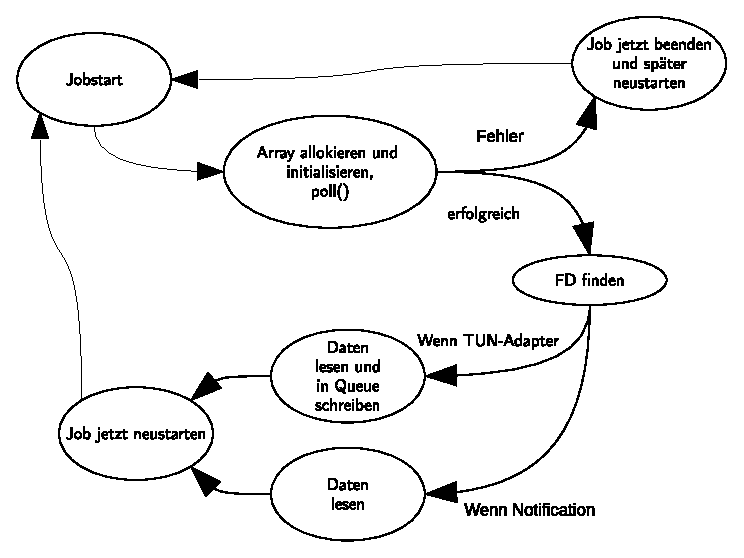
\includegraphics[width=\textwidth]{poll_fd.eps}
\end{figure}

Folgend die originale Implementierung für Linux und Unix mit poll()
% Stattdessen Pseudocode?
\begin{lstlisting}[caption=Code für handle\_plain auf Unix/Linux]
/**
 * Job handling outbound plaintext packets
 */
static job_requeue_t handle_plain(private_kernel_libipsec_router_t *this)
{
	enumerator_t *enumerator;
	tun_entry_t *entry;
	bool oldstate;
	int count = 0;
	char buf[1];
	struct pollfd *pfd;

	this->lock->read_lock(this->lock);

	pfd = alloca(sizeof(*pfd) * (this->tuns->get_count(this->tuns) + 2));
	pfd[count].fd = this->notify[0];
	pfd[count].events = POLLIN;
	count++;
	pfd[count].fd = this->tun.fd;
	pfd[count].events = POLLIN;
	count++;

	enumerator = this->tuns->create_enumerator(this->tuns);
	while (enumerator->enumerate(enumerator, NULL, &entry))
	{
		pfd[count].fd = entry->fd;
		pfd[count].events = POLLIN;
		count++;
	}
	enumerator->destroy(enumerator);
	this->lock->unlock(this->lock);

	oldstate = thread_cancelability(TRUE);
	if (poll(pfd, count, -1) <= 0)
	{
		thread_cancelability(oldstate);
		return JOB_REQUEUE_FAIR;
	}
	thread_cancelability(oldstate);

	if (pfd[0].revents & POLLIN)
	{
		/* list of TUN devices changed, read notification data, rebuild FDs */
		while (read(this->notify[0], &buf, sizeof(buf)) == sizeof(buf))
		{
			/* nop */
		}
		return JOB_REQUEUE_DIRECT;
	}

	if (pfd[1].revents & POLLIN)
	{
		process_plain(this->tun.tun);
	}

	this->lock->read_lock(this->lock);
	enumerator = this->tuns->create_enumerator(this->tuns);
	while (enumerator->enumerate(enumerator, NULL, &entry))
	{
		if (find_revents(pfd, count, entry->fd) & POLLIN)
		{
			process_plain(entry->tun);
		}
	}
	enumerator->destroy(enumerator);
	this->lock->unlock(this->lock);

	return JOB_REQUEUE_DIRECT;
}
\end{lstlisting}

Wie aus dem Code hervorgeht, wird im Prinzip nur ein Array mit Strukturen des Typs
''pollfd'' erstellt, dann mit einem Notification-\ac{FD} und den \acp{FD} der TUN-Geräte befüllt
und als gewünschte Events ''POLLIN'' gesetzt. Das heißt, dass der Aufruf von poll() ohne
Fehler beendet wird, wenn Daten auf dem \acp{FD} zur Verfügung stehen.
Danach wird poll() auf die ''pollfd''-Datenstruktur ausgeführt und analysiert,
auf welchen \acp{FD} Daten zur Verfügung stehen.

Folgend die Implementierung mit WaitForMultipleObjects()
\begin{lstlisting}[caption=Code für handle\_plain auf Windows]
static job_requeue_t handle_plain(private_kernel_libipsec_router_t *this)
{
        DBG1(DBG_LIB, "entered handle_plain.");
        void **key = NULL;
        bool oldstate, status;
        uint32_t length, event_status = 0, i = 0, j = 0;
        handle_overlapped_buffer_t *bundle_array = NULL, dummy, tun_device_handle_overlapped_buffer, *structures = NULL;
        OVERLAPPED *overlapped = NULL;
        HANDLE *event_array = NULL, tun_device_event;
        tun_device_t *tun_device = this->tun.tun;
        enumerator_t *tuns_enumerator;

        memset(&tun_device_handle_overlapped_buffer, 0, sizeof(handle_overlapped_buffer_t));
        /* Reset synchronisation event */
        ResetEvent(this->event);

        length = this->tuns->get_count(this->tuns);

        this->lock->read_lock(this->lock);
        /* Read event for this->tun */

        /* allocate arrays for all the structs we need */
        /* events, overlapped structures and bundles. */
        /* event_array holds all the HANDLE structures for the events that are
         * used for notifying the thread of finished reads and writes.
         */

        overlapped = alloca((length+2)*sizeof(OVERLAPPED));
        event_array = alloca((length+2)*sizeof(HANDLE));
        bundle_array = alloca((length+2)*sizeof(handle_overlapped_buffer_t));

        memset(overlapped, 0, (length+2)*sizeof(OVERLAPPED));
        memset(bundle_array, 0, (length+2)*sizeof(handle_overlapped_buffer_t));

        DBG1(DBG_LIB, "Allocated arrays, opened events");

        /* These are the arrays we're going to work with */

        /* first position is the event we use for synchronisation  */
        /* Insert notification event */
        event_array[i] = this->event;
        /* Insert dummy structure */
        bundle_array[i] = dummy;
        i++;

        /* second position is this->tun */
        /* insert event object for this->tun device */
        tun_device_event = CreateEvent(NULL, FALSE, FALSE, this->tun.tun->get_read_event_name(this->tun.tun));
        if (!tun_device_event)
        {
            DWORD error = GetLastError();
            char *lpMsgBuf;
            FormatMessage(
                FORMAT_MESSAGE_ALLOCATE_BUFFER |
                FORMAT_MESSAGE_FROM_SYSTEM |
                FORMAT_MESSAGE_IGNORE_INSERTS,
                NULL,
                error,
                MAKELANGID(LANG_NEUTRAL, SUBLANG_DEFAULT),
                (LPTSTR) &lpMsgBuf,
                0, NULL );
            DBG1(DBG_LIB, "Error: %s", lpMsgBuf);
            raise(SIGTERM);
        }
        event_array[i] = tun_device_event;
        ResetEvent(event_array[i]);
        /* bundle for the read on this->tun */
        /* Reserve memory for the buffer*/
        tun_device_handle_overlapped_buffer.buffer = chunk_alloca(tun_device->get_mtu(tun_device));
        DBG1(DBG_LIB, "Allocated buffer.");
        tun_device_handle_overlapped_buffer.fileHandle = tun_device->get_handle(tun_device);
        DBG1(DBG_LIB, "Allocated file handle.");
        tun_device_handle_overlapped_buffer.overlapped = overlapped;
        DBG1(DBG_LIB, "Allocated overlapped..");
        /* Fill in code */
        tun_device_handle_overlapped_buffer.overlapped->hEvent = OpenEvent(EVENT_ALL_ACCESS, FALSE, this->tun.tun->get_read_event_name(this->tun.tun));
        if (tun_device_handle_overlapped_buffer.overlapped->hEvent == NULL)
        {
            DWORD error = GetLastError();
            char *lpMsgBuf;
            FormatMessage(
                FORMAT_MESSAGE_ALLOCATE_BUFFER |
                FORMAT_MESSAGE_FROM_SYSTEM |
                FORMAT_MESSAGE_IGNORE_INSERTS,
                NULL,
                error,
                MAKELANGID(LANG_NEUTRAL, SUBLANG_DEFAULT),
                (LPTSTR) &lpMsgBuf,
                0, NULL );
            DBG1(DBG_LIB, "Error: %s", lpMsgBuf);
            raise(SIGTERM);
        }
        DBG1(DBG_LIB, "Created event");
        bundle_array[i] = tun_device_handle_overlapped_buffer;

        DBG1(DBG_LIB, "%d", tun_device_handle_overlapped_buffer.buffer.ptr[1499]);
        DBG1(DBG_LIB, "handle: %d", tun_device_handle_overlapped_buffer.fileHandle);
        DBG1(DBG_LIB, "%d", tun_device_handle_overlapped_buffer.overlapped->hEvent);
        i++;

        /* Start ReadFile for this->tun.handle */
        status = ReadFile(tun_device_handle_overlapped_buffer.fileHandle,
            tun_device_handle_overlapped_buffer.buffer.ptr,
            tun_device_handle_overlapped_buffer.buffer.len,
            NULL,
            tun_device_handle_overlapped_buffer.overlapped );
        if (status)
        {
            SetEvent(tun_device_handle_overlapped_buffer.overlapped->hEvent);
        }
        else
        {
            DWORD error = GetLastError();
            switch(error)
            {
                case ERROR_IO_PENDING:
                    /* IO enqueud. Everything's fine. */
                    break;
                case ERROR_INVALID_USER_BUFFER:
                case ERROR_NOT_ENOUGH_MEMORY:
                    /* too many outstanding I/O requests
                     * We can't fix that and need to stop the process
                     */
                    DBG1(DBG_LIB, "the operating system did not allow us to enqueue more asynchronous operations");
                    this->lock->unlock(this->lock);
                    raise(SIGTERM);
                    /* fatal error */
                    break;
                case ERROR_NOT_ENOUGH_QUOTA:
                    /* unable to page lock calling process's buffer */
                    DBG1(DBG_LIB, "the operating system could not lock the buffer");
                    this->lock->unlock(this->lock);
                    /* fatal error */
                    raise(SIGTERM);
                    break;
                default:
                    DBG1(DBG_LIB, "Unknown error %d occured", error);
                    /* Some error we don't know */
                    /* exit */
                    /* TODO: Translate error number to human readable*/
                    /* fatal error */
                    raise(SIGTERM);
                    break;
            }

        }
        /* pad bundle_array with two empty structures */
        /* iterate over all our tun devices, create event handles, reset them, queue read operations on all handles */

        DBG1(DBG_LIB, "Enumerating tun devices ...");

        tuns_enumerator = this->tuns->create_enumerator(this->tuns);
        while(tuns_enumerator->enumerate(tuns_enumerator, key, &tun_device))
        {
            /* Allocate structure and buffer */

            structures[j].buffer = chunk_alloca(tun_device->get_mtu(tun_device));
            structures[j].fileHandle = tun_device->get_handle(tun_device);
            /* Allocate and initialise OVERLAPPED structure */
            structures[j].overlapped = alloca(sizeof(OVERLAPPED));
            (*structures[j].overlapped) = overlapped[j];
            memset(&structures[j].overlapped, 0, sizeof(OVERLAPPED));
            /* Create unique name for that event. */
            /* Create unique event for read accesses on that device
             * No security attributes, no manual reset, initial state is unsignaled,
             * name is the special name we created
             */
            structures[j].overlapped->hEvent = CreateEvent(NULL, FALSE, FALSE, tun_device->get_read_event_name(tun_device));
            event_array[i] = OpenEvent(EVENT_ALL_ACCESS, FALSE, tun_device->get_read_event_name(tun_device));
            bundle_array[i] = structures[j];

            if (event_array[i] == NULL)
            {
                DWORD error = GetLastError();
                char *lpMsgBuf;
                FormatMessage(
                    FORMAT_MESSAGE_ALLOCATE_BUFFER |
                    FORMAT_MESSAGE_FROM_SYSTEM |
                    FORMAT_MESSAGE_IGNORE_INSERTS,
                    NULL,
                    error,
                    MAKELANGID(LANG_NEUTRAL, SUBLANG_DEFAULT),
                    (LPTSTR) &lpMsgBuf,
                    0, NULL );
                DBG1(DBG_LIB, "Error: %s", lpMsgBuf);
                raise(SIGTERM);
            }
            i++;

            /* Initialise read with the allocate overwrite structure */
            DBG1(DBG_LIB, "Reading on %s", tun_device->get_name(tun_device));
            status = ReadFile(structures[j].fileHandle, structures[j].buffer.ptr,
                    structures[j].buffer.len, NULL, structures[j].overlapped);
            if (status)
            {
                /* Read returned immediately */
                /* We need to signal the event ourselves */

                SetEvent(event_array[i]);
                continue;
            }
            else
            {
                DWORD error = GetLastError();
                switch(error)
                {
                    case ERROR_IO_PENDING:
                        /* IO enqueud. Everything's fine. */
                        break;
                    case ERROR_INVALID_USER_BUFFER:
                    case ERROR_NOT_ENOUGH_MEMORY:
                        /* too many outstanding I/O requests
                         * We can't fix that and need to stop the process
                         */
                        DBG1(DBG_LIB, "the operating system did not allow us to enqueue more asynchronous operations");
                        this->lock->unlock(this->lock);
                        raise(SIGTERM);
                        /* fatal error */
                        break;
                    case ERROR_NOT_ENOUGH_QUOTA:
                        /* unable to page lock calling process's buffer */
                        DBG1(DBG_LIB, "the operating system could not lock the buffer");
                        this->lock->unlock(this->lock);
                        /* fatal error */
                        raise(SIGTERM);
                        break;
                    default:
                        DBG1(DBG_LIB, "Unknown error %d occured", error);
                        /* Some error we don't know */
                        /* exit */
                        /* TODO: Translate error number to human readable*/
                        /* fatal error */
                        raise(SIGTERM);
                        break;
                }
            }
            j++;
        }
        tuns_enumerator->destroy(tuns_enumerator);

        this->lock->unlock(this->lock);

        while(TRUE)
        {
            /* Wait for a handle to be signaled */
            /* In the mingw64 sources, MAXIMUM_WAIT_OBJECTS is defined as 64. That means we can wait for a maximum of 64 event handles.
             * This translates to 63 tun devices. I think this is sufficiently high to not have to implement a mechanism for waiting for more
             * events /support more TUN devices */
            oldstate = thread_cancelability(FALSE);
            DBG1(DBG_LIB, "Waiting for events...");
            event_status = WaitForMultipleObjects(i, event_array, FALSE, INFINITE);
            thread_cancelability(oldstate);
            DBG1(DBG_LIB, "Event triggered...");
            /* A handle was signaled. Find the tun handle whose read was successful */

            /* We can only use the event_status of indication for the first completed IO operation.
             * After the event was signaled, we need to test the OVERLAPPED structure in the other array
             * to find out what event was signaled.
             */

            if ((WAIT_OBJECT_0 < event_status) < ((WAIT_OBJECT_0 + length - 1)))
            {
                /* the event at event_array[event_status - WAIT_OBJECT_0] has been signaled */
                /* It is possible that more than one event was signalled. In that case, (event_status - WAIT_OBJECT_0)
                 * is the index with the lowest event that was signalled. More signalled events can be found higher
                 */
                DWORD offset = event_status - WAIT_OBJECT_0;
                if (offset == 0)
                {
                    /* Notification about changes regarding the tun devices.
                     * We need to rebuild the array. So exit and rebuild. */
                    DBG1(DBG_LIB, "cleanup.");
                    /* Cleanup*/
                    for(uint32_t k=0;k<i;k++)
                    {
                        /* stop all asynchronous IO */
                        CancelIo(bundle_array[k].fileHandle);
                        CloseHandle(bundle_array[k].overlapped->hEvent);
                        ResetEvent(event_array[k]);
                        CloseHandle(event_array[k]);
                    }
                    /* exit */
                    DBG1(DBG_LIB, "Cleanup done.");
                    return JOB_REQUEUE_FAIR;
                }
                for(uint32_t k=1;k<i; k++)
                {
                    /* Is the object signaled? */
                    DBG1(DBG_LIB, "checking if event is signaled.");
                    if (WaitForSingleObject(event_array[k], 0) == WAIT_OBJECT_0)
                    {
                        /* The arrays have the same length and the same positioning of the elements.
                         * Therefore, if event_array[k] is signaled, the read on bundle_array[i].fileHandle has succeeded
                         * and bundle_array[k].buffer has our data now. */

                        /* Do we need to copy the chunk before we enqueue it? */
                        DBG1(DBG_LIB, "Event is signaled. Processing packet.");
                        ip_packet_t *packet;
                        packet = ip_packet_create(bundle_array[k].buffer);
                        if (packet)
                        {
                                ipsec->processor->queue_outbound(ipsec->processor, packet);
                        }
                        else
                        {
                                DBG1(DBG_KNL, "invalid IP packet read from TUN device");
                        }
                        /* Reset the overlapped structure, event and buffer */
                        memset(&bundle_array[k].overlapped, 0, sizeof(OVERLAPPED));
                        /* Don't leak packets */
                        memset(bundle_array[k].buffer.ptr, 0, bundle_array[k].buffer.len);

                        bundle_array[k].overlapped->hEvent = event_array[k];
                        ResetEvent(event_array[k]);

                    }
                }

            }
            /* Function failed */
            else
            {
                DBG1(DBG_LIB, "waiting for events on the tun device reads failed.");
                /* cleanup, exit, retry */
            }
        }

        return JOB_REQUEUE_DIRECT;
}
\end{lstlisting}

libipsec setzt für die von ihr installierten Routen standardmäßig das ''Gateway''
oder ''Next Hop''Feld nicht. Der Grund dafür ist, dass libipsec bisher nur auf
Betriebssytemen genutzt wurde, die echte Layer-3-Geräte implementieren und
daher keine Kollisionsdomäne über das Gerät erreichbar ist. Daher ergibt es keinen
Sinn das ''next hop''-Feld zu setzen.
Auf Windows ist dies jedoch, wie zuvor erläutert, nicht der Fall, da der TAP-Windows-Treiber
TUN-Geräte als Ethernet-Gerät emuliert.
\begin{lstlisting}[caption=Patch für die Routen-Installation von libipsec]
#ifdef __linux__
#elif defined(WIN32)
        /* TODO: Complete */
        /* Set out special gateway */
        /* We also need to add a route to 169.254.0.0/16 via all our tun devices */
        host_t *gw = host_create_from_string("169.254.128.128", 0);
        route->gateway = gw;
#else
	/* on Linux we cant't install a gateway */
	route->gateway = charon->kernel->get_nexthop(charon->kernel, dst, -1, src);
#endif
\end{lstlisting}
% libipsec router
% handle_plain
% notification event
% job
% handle_plain
% handle_esp
% up
% destroy
%kernel_libipsec_ipsec route installation
\subsubsection{libstrongswan}
Hier galt es das Öffnen, Konfigurieren und Schließen von TUN-Geräten
mit dem TAP-Windows-Treiber zu implementieren.

% Bezugsquelle für den Treiber
Der Treiber ist kompiliert auf der OpenVPN-Seite
verfügbar\footnote{\url{https://openvpn.net/index.php/open-source/downloads.html}}
und der Quellcode auf Github\footnote{\url{https://github.com/OpenVPN}}.
Die Basis für die Implementierung war hier der existierende Programmcode in
OpenVPN, spezifisch in Datei /src/openvpn/tun.c.

Um das TAP-Gerät zu nutzen versucht der Code zuerst nach Netzwerkgeräten mit der ID "tap0901" zu suchen,
welche die ID für TAP-Geräte ist.

Danach wird versucht eine Datei in \\.\\Global\/GUID.tap mittels 
\begin{lstlisting}
CreateFile(device_path, GENERIC_READ \| GENERIC_WRITE, 0,
                    0, OPEN_EXISTING, FILE_ATTRIBUTE_SYSTEM | FILE_FLAG_OVERLAPPED, 0);
\end{lstlisting}
zu öffnen.
Das Handle kann nun genutzt werden um Pakete vom TAP-Gerät zu lesen und zu schreiben.
Mittels DeviceIoControl kann die Konfiguration des Geräts geändert werden,
wie die IP des virtuellen Routers, den Status des Geräts sowie der Modus des Geräts.

Für die Portierung wurden die \acp{FD} für Handles ausgetauscht und für das Benachrichtigen
über Änderungen in der Liste der TUN-Geräte wurde ein Event verwendet.

Da Eventbasiertes IO-Multiplexing genutzt wird, werden verschiedene Events zum Lesen
und Schreiben verwendet.
Die Namen der Events werden als Attribut des Objekts in ''tun\_device\_t->read\_event\_name''
''tun\_device\_t->write\_event\_name'' gespeichert. Sie können mittles ''tun\_device\_t->get\_read\_event\_name()'
und ''tun\_device\_t->get\_read\_event\_name()'' gelesen werden.

\begin{lstlisting}[caption=Code für das Suchen eines TAP-Geräts]
/*
 * Searches through the registry for suitable TAP driver interfaces
 * On Windows, the TAP interface metadata is stored and described in the registry.
 * It returns a linked list that contains all found guids. The guids describe the interfaces.
 */

linked_list_t *get_tap_reg()
{
    HKEY adapter_key;
    LONG status;
    DWORD len;
    linked_list_t *list = linked_list_create();
    int i = 0;

    /*
     * Open parent key. It contains all other keys that
     * describe any possible interfaces.
     */
    status = RegOpenKeyEx(
            HKEY_LOCAL_MACHINE,
            ADAPTER_KEY,
            0,
            KEY_READ,
            &adapter_key);

    if (status != ERROR_SUCCESS)
    {
        DBG2(DBG_LIB, "Error opening registry key: %s", ADAPTER_KEY);
    }

    while (true)
    {
        char enum_name[256];
        char unit_string[256];
        HKEY unit_key;
        char component_id_string[] = "ComponentId";
        char component_id[256];
        char net_cfg_instance_id_string[] = "NetCfgInstanceId";
        char net_cfg_instance_id[256];
        DWORD data_type;

        len = sizeof (enum_name);
        status = RegEnumKeyEx(
                adapter_key,
                i,
                enum_name,
                &len,
                NULL,
                NULL,
                NULL,
                NULL);
        if (status == ERROR_NO_MORE_ITEMS)
        {
            break;
        }
        else if (status != ERROR_SUCCESS)
        {
            DBG2(DBG_LIB, "Error enumerating registry subkeys of key: %s",
                    ADAPTER_KEY);
        }

        snprintf(unit_string, sizeof (unit_string), "%s\\%s",
                ADAPTER_KEY, enum_name);

        status = RegOpenKeyEx(
                HKEY_LOCAL_MACHINE,
                unit_string,
                0,
                KEY_READ,
                &unit_key);

        if (status != ERROR_SUCCESS)
        {
            DBG2(DBG_LIB, "Error opening registry key: %s", unit_string);
        }
        else
        {
            len = sizeof (component_id);
            status = RegQueryValueEx(
                    unit_key,
                    component_id_string,
                    NULL,
                    &data_type,
                    component_id,
                    &len);

            if (status != ERROR_SUCCESS || data_type != REG_SZ)
            {
                DBG2(DBG_LIB, "Error opening registry key: %s\\%s",
                        unit_string, component_id_string);
            }
            else
            {
                len = sizeof (net_cfg_instance_id);
                status = RegQueryValueEx(
                        unit_key,
                        net_cfg_instance_id_string,
                        NULL,
                        &data_type,
                        net_cfg_instance_id,
                        &len);

                if (status == ERROR_SUCCESS && data_type == REG_SZ)
                {
                    if (!strcmp(component_id, TAP_WIN_COMPONENT_ID))
                    {
                        /* That thing is a valid interface key */
                        /* link into return list */
                        char *guid = malloc(sizeof(net_cfg_instance_id));
                        memcpy(guid, net_cfg_instance_id, sizeof(net_cfg_instance_id));
                        list->insert_last(list, guid);
                    }
                }
            }
            RegCloseKey(unit_key);
        }
        ++i;
    }

    RegCloseKey(adapter_key);
    return list;
}
\end{lstlisting}

Folgend ist der Code für das Konfigurieren eines TAP-Geräts:
\begin{lstlisting}[caption=Konfiguration eines TAP-Geräts]
/**
 * Initialize the tun device
 */
static bool init_tun(private_tun_device_t *this, const char *name_tmpl)
[...]
#elif defined(WIN32)
        /* WIN32 TAP driver stuff*/
        /* Check if there is an unused tun device following the IPsec name scheme*/
        enumerator_t *enumerator;
        char *guid;
        BOOL success = FALSE;
        linked_list_t *possible_devices = get_tap_reg();
        memset(this->if_name, 0, sizeof(this->if_name));

        this->read_event_name = malloc(WIN32_TUN_EVENT_LENGTH);
        this->write_event_name = malloc(WIN32_TUN_EVENT_LENGTH);
        /* Iterate over list */
        enumerator = possible_devices->create_enumerator(possible_devices);
        /* Try to open that device */
        while(enumerator->enumerate(enumerator, &guid))
        {
            if (!success){
                /* Set mode */
                char device_path[256];
                /* Translate dev name to guid */
                /* TODO: Fix. device_guid should be */
                snprintf (device_path, sizeof(device_path), "%s%s%s", USERMODEDEVICEDIR, guid, TAP_WIN_SUFFIX);

                this->tunhandle = CreateFile(device_path, GENERIC_READ | GENERIC_WRITE, 0,
                    0, OPEN_EXISTING, FILE_ATTRIBUTE_SYSTEM | FILE_FLAG_OVERLAPPED, 0);
                if (this->tunhandle == INVALID_HANDLE_VALUE)
                {
                    DBG1(DBG_LIB, "could not create TUN device %s", device_path);
                }
                else
                {
                    memcpy(this->if_name, guid, strlen(guid));
                    success = TRUE;
                }
            }
            else
            {
                break;
            }
            /* device has been examined or used, free it */
            free(guid);
        }

        /* possible_devices has been freed while going over the enumerator.
         * Therefore it is not necessary to free the elements in the list now.
         */
        enumerator->destroy(enumerator);
        possible_devices->destroy(possible_devices);
        if (!success)
        {
            return FALSE;
        }
        /* set correct mode */
        /* We set a fake gateway of 169.254.254.128 that we route packets over
         The TAP driver strips the Ethernet header and trailer of the Ethernet frames
         before sending them back to the application that listens on the handle */
	struct in_addr ep[3];
        ULONG status = TRUE;
        DWORD len;
        /* Local address (just fake one): 169.254.128.127 */
	ep[0].S_un.S_un_b.s_b1 = 169;
        ep[0].S_un.S_un_b.s_b2 = 254;
        ep[0].S_un.S_un_b.s_b3 = 128;
        ep[0].S_un.S_un_b.s_b4 = 127;
        /*
         * Remote network. The tap driver validates it by masking it with the remote_netmask
         * and then comparing hte result against the remote network (this value here).
         * If it does not match, an error is logged and initialization fails.
         * (local & remote_netmask ? local)
         * The driver does proxy arp for this network and the local address.
         */
        /* We need to integrate support for IPv6, too. */
        /* Just fake a link local address for now (169.254.128.128) */
	ep[1].S_un.S_un_b.s_b1 = 169;
        ep[1].S_un.S_un_b.s_b2 = 254;
        ep[1].S_un.S_un_b.s_b3 = 128;
        ep[1].S_un.S_un_b.s_b4 = 128;
        /* Remote netmask (255.255.255.255) */
	ep[2].S_un.S_un_b.s_b1 = 255;
        ep[2].S_un.S_un_b.s_b2 = 255;
        ep[2].S_un.S_un_b.s_b3 = 255;
        ep[2].S_un.S_un_b.s_b4 = 255;

        if(!DeviceIoControl (this->tunhandle, TAP_WIN_IOCTL_CONFIG_TUN,
		    ep, sizeof (ep),
		    ep, sizeof (ep), &len, NULL))
        {
            DBG1 (DBG_LIB, "WARNING: The TAP-Windows driver rejected a TAP_WIN_IOCTL_CONFIG_TUN DeviceIoControl call.");
        }

        ULONG disable_src_check = FALSE;
        if(!DeviceIoControl(this->tunhandle, TAP_WIN_IOCTL_CONFIG_SET_SRC_CHECK,
                    &disable_src_check, sizeof(disable_src_check),
                    &disable_src_check, sizeof(disable_src_check), &len, NULL))
        {
            DBG1 (DBG_LIB, "WARNING: The TAP-Windows driver rejected a TAP_WIN_IOCTL_CONFIG_SET_SRC_CHECK DeviceIoControl call.");
        }
        ULONG driverVersion[3] = {0 , 0, 0};
        if(!DeviceIoControl(this->tunhandle, TAP_WIN_IOCTL_GET_VERSION,
                    &driverVersion, sizeof(driverVersion),
                    &driverVersion, sizeof(driverVersion), &len, NULL))
        {
            DBG1(DBG_LIB, "WARNING: The TAP-Windows driver rejected a TAP_WIN_IOCTL_GET_VERSION DeviceIoControl call.");
        }
        else
        {
            DBG1(DBG_LIB, "TAP-Windows driver version %d.%d available.", driverVersion[0], driverVersion[1]);
        }
        /* Set device to up */

        if (!DeviceIoControl (this->tunhandle, TAP_WIN_IOCTL_SET_MEDIA_STATUS,
  			  &status, sizeof (status),
                            &status, sizeof (status), &len, NULL))
        {
            DBG1 (DBG_LIB, "WARNING: The TAP-Windows driver rejected a TAP_WIN_IOCTL_SET_MEDIA_STATUS DeviceIoControl call.");
        }

            /* Give the adapter 2 seconds to come up */
        /* Create event with special template */
        snprintf(this->read_event_name, WIN32_TUN_EVENT_LENGTH, WIN32_TUN_READ_EVENT_TEMPLATE, this->if_name);
        snprintf(this->write_event_name, WIN32_TUN_EVENT_LENGTH, WIN32_TUN_WRITE_EVENT_TEMPLATE, this->if_name);
        sleep(2);
        return TRUE;
        [...]
}
\end{lstlisting}

Für das Setzen des Geräts auf ''up'' wurde der entsprechende Aufruf per IoControl
implementiert:
\begin{lstlisting}[caption=Code für das Setzen des Geräts auf ''up'']
/* Fix for WIN32 */
METHOD(tun_device_t, up, bool,
	private_tun_device_t *this)
{
#ifdef WIN32
        ULONG status = TRUE;
        DWORD len;
        if (!DeviceIoControl (this->tunhandle, TAP_WIN_IOCTL_SET_MEDIA_STATUS,
			  &status, sizeof (status),
			  &status, sizeof (status), &len, NULL))
        {
            DBG1(DBG_LIB, "failed to set the interface %s to up", this->if_name);
            return FALSE;
        }
#else
        [...]
#endif /* WIN32 */
	return TRUE;
}
\end{lstlisting}

Folgend der Code für das Erstellen eines Objects vom Typ ''tun\_device\_t''.

\begin{lstlisting}[caption=Code für das Erstellen von tun\_device\_t]
/*
 * Described in header
 */
tun_device_t *tun_device_create(const char *name_tmpl)
{
	private_tun_device_t *this;

	INIT(this,
		.public = {
			.read_packet = _read_packet,
			.write_packet = _write_packet,
			.get_mtu = _get_mtu,
			.set_mtu = _set_mtu,
			.get_name = _get_name,
                        /* For WIN32, that's a handle. */
#ifdef WIN32
                        .get_handle = _get_handle,
                        .get_write_event_name = _get_write_event_name,
                        .get_read_event_name = _get_read_event_name,
#else
			.get_fd = _get_fd,
#endif /* WIN32 */
			.set_address = _set_address,
			.get_address = _get_address,
			.up = _up,
			.destroy = _destroy,
		},
#ifdef WIN32
                .tunhandle = NULL,
#else
		.tunfd = -1,
		.sock = -1,
#endif /* WIN32 */
	);

	if (!init_tun(this, name_tmpl))
	{
		free(this);
		return NULL;
	}
	DBG1(DBG_LIB, "created TUN device: %s", this->if_name);

#ifdef WIN32
#else
	this->sock = socket(AF_INET, SOCK_DGRAM, 0);
	if (this->sock < 0)
	{
		DBG1(DBG_LIB, "failed to open socket to configure TUN device");
		destroy(this);
		return NULL;
	}
#endif /* WIN32 */
	return &this->public;
}

#endif /* TUN devices supported */
\end{lstlisting}

\begin{lstlisting}[caption=Relevanter code für tun\_device\_t->destroy()]
METHOD(tun_device_t, destroy, void,
	private_tun_device_t *this)
{
#ifdef WIN32
        /* close file handle, destroy interface */
        CloseHandle(this->tunhandle);
        free(this->read_event_name);
        free(this->write_event_name);
#else
        [...]
#endif
    	DESTROY_IF(this->address);
    	free(this);
}
\end{lstlisting}
% callbacks
% synchronous
% WaitForMultipleObjects
% komplexe Änderungen des Verhaltens von kernel-libipsec

\subsubsection{kernel-iph}
kernel-iph ist ein Plugin für charon, das das Kernel-Interface
für die Verwaltung von IP-Adressen und Routen implementiert.

Ursprünglich war das Verwalten von IP-Adressen im Master-Zweig nicht implementiert.
Eine vollständige Implementierung existiert im Zweig "win-vip", die in den Zweig 'windows-libipsec'
gemerged wurde, um eine vollständige Implementierung dort zu erhalten.
%TODO: Codebeispiele?
Nachgerüstet werden musste Code zum Beachten des "charon.install\_virtual\_ip\_on" Parameters
der in der Datei "strongswan.conf" definiert werden kann und den libipsec nutzt um
die Installation der empfangenen IP-Adresse(n) auf den richtigen Adapter zu erzwingen.
Der Code kopiert den Adapternamen während der Initialisierung des Plugins, daher
ändert ein Ändern des Parameters während der Laufzeit nicht die Schnittstelle,
auf die die IP-Adresse installiert werden würde.

Die bekannten IP-Adressen werden in kernel-iph in einer Datenstruktur gespeichert,
um sie schnell nachschlagen zu können und Berechnungen zu tätigen. Die Struktur
wird einerseits durch manuelles Einfügen und Entfernen von selbstinstallierten Adressen
bewerkstelligt, als auch durch Events, die der Kernel per 

\begin{lstlisting}[caption=Ergänzung zu private\_kernel\_iph\_net\_t]
/**
 * Private data of kernel_iph_net implementation.
 */
struct private_kernel_iph_net_t {
        [...]
        /**
         * Whether to install virtual IPs
         */
        bool install_virtual_ip;

        /**
         * Where to install virtual IPs
         */

        char *install_virtual_ip_on;
};
\end{lstlisting}

\begin{lstlisting}[caption=Code für add\_ip]
METHOD(kernel_net_t, add_ip, status_t,
	private_kernel_iph_net_t *this, host_t *vip, int prefix, char *name)
{
	if (!this->install_virtual_ip)
	{	/* disabled by config */
		return SUCCESS;
	}
	MIB_UNICASTIPADDRESS_ROW row;
	u_long status;
        iface_t *iface = NULL, *entry = NULL;

        /* Print out all known interfaces */
        enumerator_t *enumerator = this->ifaces->create_enumerator(this->ifaces);
        while(enumerator->enumerate(enumerator, &entry))
        {
            DBG1(DBG_KNL, "interface %s\n index: %d\n description %s\n type %d", entry->ifname, entry->ifindex, entry->ifdesc, entry->iftype);
        }
        enumerator->destroy(enumerator);
	/* name of the MS Loopback adapter */
        if (!this->install_virtual_ip_on || this->ifaces->find_first(this->ifaces, (void*)iface_by_name,
						(void**)&iface, this->install_virtual_ip_on) != SUCCESS)
        {
            name = "{DB2C49B1-7C90-4253-9E61-8C6A881194ED}";
        }
        else
        {
            name = this->install_virtual_ip_on;
        }
	host2unicast(vip, prefix, &row);

	row.InterfaceIndex = add_addr(this, name, vip, TRUE);
	if (!row.InterfaceIndex)
	{
		DBG1(DBG_KNL, "interface '%s' not found", name);
		return NOT_FOUND;
	}

	status = CreateUnicastIpAddressEntry(&row);
	if (status != NO_ERROR)
	{
		DBG1(DBG_KNL, "creating IPH address entry failed: %lu", status);
		remove_addr(this, vip);
		return FAILED;
	}
	return SUCCESS;
}
\end{lstlisting}

\begin{lstlisting}[caption=Code für del\_ip]
METHOD(kernel_net_t, del_ip, status_t,
	private_kernel_iph_net_t *this, host_t *vip, int prefix, bool wait)
{
        if (!this->install_virtual_ip)
	{	/* disabled by config */
		return SUCCESS;
	}

	MIB_UNICASTIPADDRESS_ROW row;
	u_long status;

	host2unicast(vip, prefix, &row);

	row.InterfaceIndex = remove_addr(this, vip);
	if (!row.InterfaceIndex)
	{
		DBG1(DBG_KNL, "virtual IP %H not found", vip);
		return NOT_FOUND;
	}

	status = DeleteUnicastIpAddressEntry(&row);
	if (status != NO_ERROR)
	{
		DBG1(DBG_KNL, "deleting IPH address entry failed: %lu", status);
		return FAILED;
	}

	return SUCCESS;
}
\end{lstlisting}

\begin{lstlisting}[caption=Ergänzung zu kernel\_iph\_net\_create()]
*
 * Described in header.
 */
kernel_iph_net_t *kernel_iph_net_create()
{
        [...}
		.install_virtual_ip = lib->settings->get_bool(lib->settings,
						"%s.install_virtual_ip", TRUE, lib->ns),
		.install_virtual_ip_on = lib->settings->get_str(lib->settings,
						"%s.install_virtual_ip_on", NULL, lib->ns),
	   [...]
}
\end{lstlisting}

Für das Implementieren des Codes für den TAP-Treiber werden Magic Numbers benötigt,
welche sich im Quellcode von OpenVPN finden lassen. Ich habe diese feig übernommen.
Teilweise habe ich auch Konstanten für die Erzeugung der Namen der Events für
das IO-Multiplexen dort abgelegt.
\begin{lstlisting}[caption=Code von win32.h]
/*
 * Copyright (C) 2016 Noel Kuntze
 *
 * Permission is hereby granted, free of charge, to any person obtaining a copy
 * of this software and associated documentation files (the "Software"), to deal
 * in the Software without restriction, including without limitation the rights
 * to use, copy, modify, merge, publish, distribute, sublicense, and/or sell
 * copies of the Software, and to permit persons to whom the Software is
 * furnished to do so, subject to the following conditions:
 *
 * The above copyright notice and this permission notice shall be included in
 * all copies or substantial portions of the Software.
 *
 * THE SOFTWARE IS PROVIDED "AS IS", WITHOUT WARRANTY OF ANY KIND, EXPRESS OR
 * IMPLIED, INCLUDING BUT NOT LIMITED TO THE WARRANTIES OF MERCHANTABILITY,
 * FITNESS FOR A PARTICULAR PURPOSE AND NONINFRINGEMENT. IN NO EVENT SHALL THE
 * AUTHORS OR COPYRIGHT HOLDERS BE LIABLE FOR ANY CLAIM, DAMAGES OR OTHER
 * LIABILITY, WHETHER IN AN ACTION OF CONTRACT, TORT OR OTHERWISE, ARISING FROM,
 * OUT OF OR IN CONNECTION WITH THE SOFTWARE OR THE USE OR OTHER DEALINGS IN
 * THE SOFTWARE.
 */

#ifndef WIN32_H
#define WIN32_H

#define WIN32_TUN_READ_EVENT_TEMPLATE "WIN32-libipsec-read-device-%d"
#define WIN32_TUN_WRITE_EVENT_TEMPLATE "WIN32-libipsec-write-device-%d"
#define WIN32_TUN_EVENT_LENGTH 80
#define TAP_WIN_COMPONENT_ID "tap0901"

#define ADAPTER_KEY "SYSTEM\\CurrentControlSet\\Control\\Class\\{4D36E972-E325-11CE-BFC1-08002BE10318}"
#define NETWORK_CONNECTIONS_KEY "SYSTEM\\CurrentControlSet\\Control\\Network\\{4D36E972-E325-11CE-BFC1-08002BE10318}"

/*
 * ======================
 * Filesystem prefixes
 * ======================
 */

#define USERMODEDEVICEDIR "\\\\.\\Global\\"
#define SYSDEVICEDIR      "\\Device\\"
#define USERDEVICEDIR     "\\DosDevices\\Global\\"
#define TAP_WIN_SUFFIX    ".tap"

/*
 * TAP IOCTL constants and macros.
 *
 */
#define TAP_WIN_CONTROL_CODE(request,method) \
  CTL_CODE (FILE_DEVICE_UNKNOWN, request, method, FILE_ANY_ACCESS)

/* Present in 8.1 */

#define TAP_WIN_IOCTL_GET_MAC               TAP_WIN_CONTROL_CODE (1, METHOD_BUFFERED)
#define TAP_WIN_IOCTL_GET_VERSION           TAP_WIN_CONTROL_CODE (2, METHOD_BUFFERED)
#define TAP_WIN_IOCTL_GET_MTU               TAP_WIN_CONTROL_CODE (3, METHOD_BUFFERED)
#define TAP_WIN_IOCTL_GET_INFO              TAP_WIN_CONTROL_CODE (4, METHOD_BUFFERED)
#define TAP_WIN_IOCTL_CONFIG_POINT_TO_POINT TAP_WIN_CONTROL_CODE (5, METHOD_BUFFERED)
#define TAP_WIN_IOCTL_SET_MEDIA_STATUS      TAP_WIN_CONTROL_CODE (6, METHOD_BUFFERED)
#define TAP_WIN_IOCTL_CONFIG_DHCP_MASQ      TAP_WIN_CONTROL_CODE (7, METHOD_BUFFERED)
#define TAP_WIN_IOCTL_GET_LOG_LINE          TAP_WIN_CONTROL_CODE (8, METHOD_BUFFERED)
#define TAP_WIN_IOCTL_CONFIG_DHCP_SET_OPT   TAP_WIN_CONTROL_CODE (9, METHOD_BUFFERED)

/* Added in 8.2 */

/* obsoletes TAP_WIN_IOCTL_CONFIG_POINT_TO_POINT */
#define TAP_WIN_IOCTL_CONFIG_TUN            TAP_WIN_CONTROL_CODE (10, METHOD_BUFFERED)
#define TAP_WIN_IOCTL_CONFIG_SET_SRC_CHECK  TAP_WIN_CONTROL_CODE (11, METHOD_BUFFERED)


#endif /* WIN32_H */
\end{lstlisting}

\subsection{Tun-Treiber}
% openvpn
% kompatibilität
% Treiber-patches upstream
Im Zuge der \ac{BA} wurde ein Patch für den TAP-Windows-Treiber entwicklelt, um die
Prüfung der Quell-IP der ARP-Requests zu deaktivieren. Das ist erforderlich, um mit der
virtuellen IP des Clients mit dem entfernten IP-Netzwerk kommunizieren zu können.
\subsubsection{Bauen und Installieren des Treibers}
Um den Treiber zu bauen, wird zuallererst der Quellcode benötigt, sowie die
Vorraussetzungen, welche auf der Github-Seite dort aufgelistet sind.
Die aktuellen Minimalvorraussetzungen sind Python 2.7, das Microsoft Windows 7 WDK (Windows Driver Kit)
und ein Windows Code signing certificate.
Das Zertifikat muss nicht valid sein, wenn der Treiber nicht produktiv ausgerollt
werden soll. Der Grund ist, dass unter Windows das Überprüfen der Treibersignatur deaktiviert
werden kann, aber der Treiber muss trotzdem signiert sein. Der Trust-path muss aber nicht
zu einem öffentlichen Trust Anchor (eine CA) führen. Um den Treiber signieren zu können,
wird die gesamte Trust Chain benötigt, sowie der private Schlüssel des Zertifikats.
Um ein Zertifikat mit dem dazugehörigen privaten Schlüssel importieren zu können,
müssen die Dateien in einen PKCS\#12-Container gepackt werden. Dieser kann mit 
OpenSSL erstellt werden, zum Beispiel mit diesem Befehl:
\begin{lstlisting}[caption=OpenSSL PKCS\#12]
openssl pkcs12 -export -in key key.key -in certificate.pem -out pkcs12.p12
\end{lstlisting}
Die mit diesem Befehl erstellte Datei pkcs12.p12 kann dann durch einen Doppelklick auf sie
in den Windows importiert werden.

Der Befehl um den Treiber dann zu bauen kann so aussehen:
\begin{lstlisting}[caption=TAP-Windows bauen]
python buildtap.py -c -b -d --cert="csc" --sign --crosscert="C:\Users\Noel\certs\rootca.pem"
\end{lstlisting}
Die Ausgabe des Befehls listet die Kompilierung, sowie das Signieren der Dateien auf.
% Hier noch Ausgabe der Kompilierung aufführen, sowie welche Teile kritisch sind.
Wie zu sehen ist, muss das Root-CA-Zertifikat als Datei vorhanden sein.
Das Code Signing certificate wird nur mit seinem Common Name angegeben.
Damit das WDK es findet, muss es in "Eigene Zertifikate" zu finden sein.
\begin{figure}
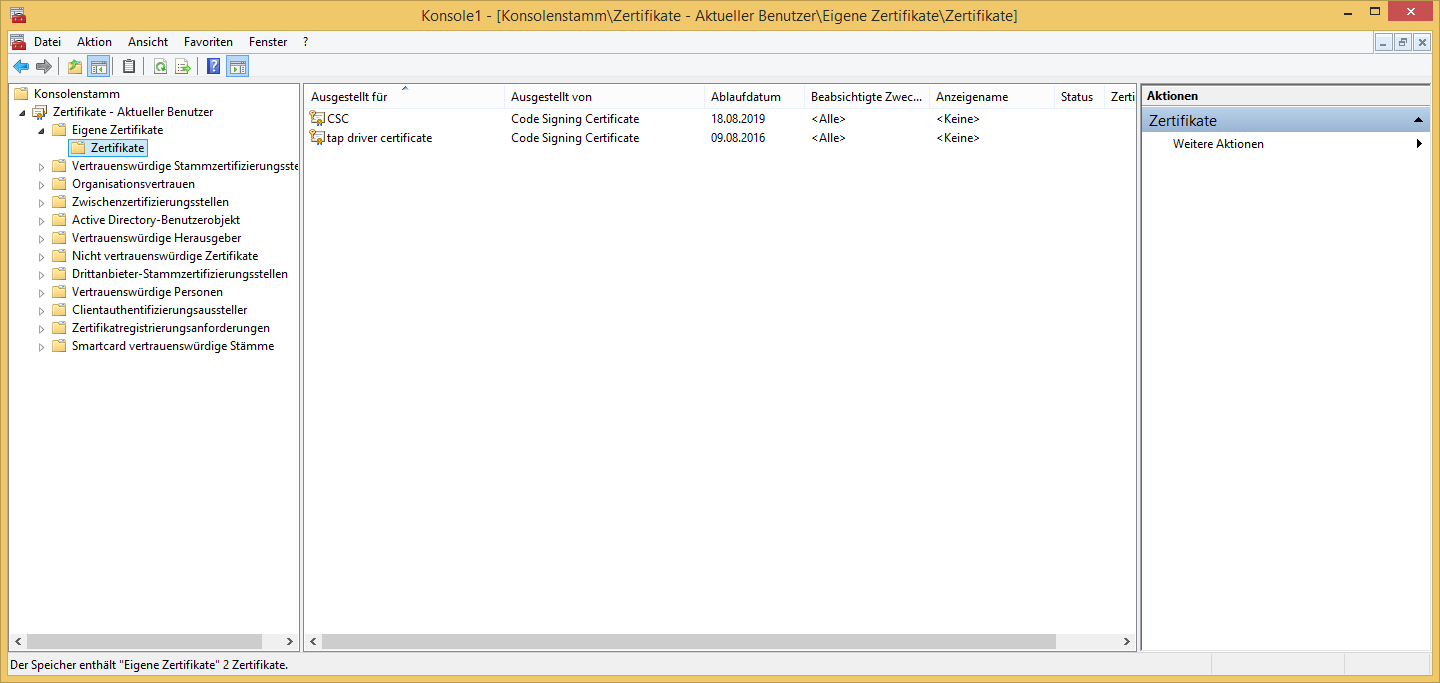
\includegraphics[scale=0.33]{/home/thermi/FH-Stuff/UNITS-8/Bachelorarbeit/Bachelorarbeit/Bilder/Eigene_Zertifikate.png}
\caption{Eigene-Zertifikate-Menü}
\label{fig:Eigene-Zertifikate-Menue}
\end{figure}

Mit Windows im Testmodus kann der Treiber geladen werden und TAP-Geräte konnen
mittels tapinstall.exe (Was eigentlich devcon.exe ist). Die Datei ist im Quellcode des
Treibers nicht mitenthalten. Sie kann jedoch durch die Installation des Treiber-Pakets
von der OpenVPN-Webseite erhalten werden. Nach der Installation des Pakets
ist die Datei unter \textit{C:\textbackslash{}Program Files\textbackslash{}TAP-Windows\textbackslash{}bin\textbackslash{}tapinstall.exe}
zu finden und kann zur Erstellung und zum Löschen von TAP-Geräten genutzt werden.

Der erste Parameter ist offensichtlich ''install'' oder ''remove''. Der Pfad zur .inf-Datei
über den Treiber muss beim Erstellen eines Geräts angegeben werden. Hier im Beispiel
ist es die Datei, die mittels des Python-Skripts erstellt wurde. Bei der Installation
dieses Treibers wird der von mir kompilierte Treiber installiert, welcher sich unter 
''C:\textbackslash{}Users\textbackslash{}Noel\textbackslash{}tap-driver\textbackslash{}dist\textbackslash{}amd64\textbackslash{}OemVista.inf''
befindet.

\begin{lstlisting}[caption=Erstellung eines TAP-Geraets]
"C:\Program Files\TAP-Windows\bin\tapinstall.exe" install "C:\Users\Noel\tap-driver\dist\amd64\OemVista.inf" tap0901
\end{lstlisting}

\begin{lstlisting}[caption=Löschung aller TAP-Geraete]
"C:\Program Files\TAP-Windows\bin\tapinstall.exe" remove tap0901
\end{lstlisting}

\paragraph{ABI}
Die \ac{ABI} des Treibers ist undokumentiert. Im Folgenden ist eine Auflistung
der Funktionen der \ac{ABI}.

\begin{table}
\tiny
\begin{tabularx}{\textwidth}{|c|c|c|c|X|X|}\firsthline
IOCtl & Makro & Eingabe & Ausgabe & Zweck & Kommentar \\ \hline
1 & TAP\_WIN\_IOCTL\_GET\_MAC & NULL & char[6] & Gibt die MAC-Adresse des Geräts zurück & \\ \hline
2 & TAP\_WIN\_IOCTL\_GET\_VERSION & NULL & ULONG[3] & Gibt die Version des Treibers zurück & \\ \hline
3 & TAP\_WIN\_IOCTL\_GET\_MTU & NULL & ULONG & Gibt die MTU des Geräts zurück & \\ \hline
4 & TAP\_WIN\_IOCTL\_GET\_INFO & NULL & N/A & Gibt Informationen über den Adapter zurück
& Ist laut Code für NDIS6 nicht implementiert \\ \hline 
5 & TAP\_WIN\_IOCTL\_CONFIG\_POINT\_TO\_POINT & IPADDR[2] (2*4 CHAR) & NULL & Setzt das Gerät in den Point-To-Point-Modus
& \\ \hline
6 & TAP\_WIN\_IOCTL\_SET\_MEDIA\_STATUS & ULONG & NULL & Setzt das Gerät in den "Up" or "Down"-Zustand & \\ \hline
7 & TAP\_WIN\_IOCTL\_CONFIG\_DHCP\_MASQ & IPADDR[4] (4*4 CHAR) & NULL & Aktiviert den internen DHCP-Server, DHCP-IP-Adresse, DHCP-Netzmaske, DHCP-Server-IP, Leasetime & \\ \hline
8 & TAP\_WIN\_IOCTL\_GET\_LOG\_LINE & allokierter String (char *) & NULL & Gibt eine Debug-Log-Zeile zurück & \\ \hline
9 & TAP\_WIN\_IOCTL\_CONFIG\_DHCP\_SET\_OPT & char[256] & NULL & Setzt die DHCP-Optionen & \\ \hline
10 & TAP\_WIN\_IOCTL\_CONFIG\_TUN & IPADDR[3] (3*4 char) & NULL & Setzt das Gerät in den TUN-Modus, lokale IP, entferntes Netzwerk, entfernte Netzmaske & \\ \hline
11 & TAP\_WIN\_IOCTL\_CONFIG\_SET\_SRC\_CHECK & ULONG & NULL & Deaktiviert oder Aktiviert den ARP-Source-Check. ''0'' deaktiviert ihn. ''1'' aktiviert ihn (Standard) & \\ \hline
\end{tabularx}
\caption{TAP-Windows-Treiber IOCtls}
\end{table}

\paragraph{Patch}
Bei der Entwicklung des Patchs wurde viel Zeit darauf verwendet die funktionalen
Komponenten zu finden, die bei der Verarbeitung von \ac{ARP}-Requests ausgeführt werden,
sowie die Codepfade zu finden, die bei der Verarbeitung von Daten abgelaufen werden.

Der entwickelte Patch deaktiviert die Überprüfung der Quell-IP der \ac{ARP}-Requests, die
vom Treiber verarbeitet werden. Wenn die Überprüfung erfolgreich war, so wird der ARP-Request
beantwortet und dem Kernel wird damit mitgeteilt, wie die MAC-Adresse des virtuellen Routers lautet.

Für die Implementierung der Routen wurde die Nutzung eines virtuellen Routers gewählt,
da das Routen aller \ac{IP}-Adressen über das Gerät die \ac{ARP}-Tabelle des Clients
mehr gefüllt hätte und eine \ac{ARP}-Adressabfrage bei jeder Kommunikation mit einer neuen
\ac{IP}-Adresse zu Folge hätte.

Er wurde 2016-08-15 in der OpenVPN Community auf freenode im Kanale \#openvpn-meeting besprochen
und bekam ein feature-ack. Ein Code-ack steht noch aus.
% https://community.openvpn.net/openvpn/ticket/721

Im folgenden ist der Patch zu finden:
\begin{lstlisting}[caption=Patch für TAP-Windows6]
diff --git a/src/adapter.c b/src/adapter.c
index 2883b79..fd575f9 100644
--- a/src/adapter.c
+++ b/src/adapter.c
@@ -222,6 +222,9 @@ tapReadConfiguration(
     Adapter->MediaStateAlwaysConnected = FALSE;
     Adapter->LogicalMediaState = FALSE;
     Adapter->AllowNonAdmin = FALSE;
+    // source check can not be set in the registry yet. This has to be set each
+    // time the adapter is opened.
+    Adapter->m_source_check = TRUE;
     //
     // Open the registry for this adapter to read advanced
     // configuration parameters stored by the INF file.
diff --git a/src/adapter.h b/src/adapter.h
index 2f09d12..70a394d 100644
--- a/src/adapter.h
+++ b/src/adapter.h
@@ -4,6 +4,7 @@
  *
  *  This code was inspired by the CIPE-Win32 driver by Damion K. Wilson.
  * 
+ *  Copyright (C) 2016 Noel Kuntze <noel@familie-kuntze.de>
  *  This source code is Copyright (C) 2002-2014 OpenVPN Technologies, Inc.,
  *  and is released under the GPL version 2 (see below).
  *
@@ -251,6 +252,10 @@ typedef struct _TAP_ADAPTER_CONTEXT
   BOOLEAN m_CalledAdapterFreeResources;
   BOOLEAN m_RegisteredAdapterShutdownHandler;
 
+   // This variable is initialised as TRUE. If it is set to FALSE, the adapter does
+   // not check the source IP field of the ARP requests it receives on the adapter.
+  BOOLEAN m_source_check;
+
 } TAP_ADAPTER_CONTEXT, *PTAP_ADAPTER_CONTEXT;
 
 FORCEINLINE
diff --git a/src/device.c b/src/device.c
index 2b7ba9b..85897b6 100644
--- a/src/device.c
+++ b/src/device.c
@@ -4,6 +4,7 @@
  *
  *  This code was inspired by the CIPE-Win32 driver by Damion K. Wilson.
  *
+ *  Copyright (C) 2016 Noel Kuntze <noel@familie-kuntze.de>
  *  This source code is Copyright (C) 2002-2014 OpenVPN Technologies, Inc.,
  *  and is released under the GPL version 2 (see below).
  *
@@ -692,7 +693,20 @@ Return Value:
             }
         }
         break;
-
+    case TAP_WIN_IOCTL_CONFIG_SET_SRC_CHECK:
+        {
+            if (inBufLength >= sizeof(ULONG))
+            {
+                adapter->m_source_check = (BOOLEAN) ((PULONG) (Irp->AssociatedIrp.SystemBuffer))[0];
+                Irp->IoStatus.Information = 1;
+            }
+            else
+            {
+                NOTE_ERROR();
+                Irp->IoStatus.Status = ntStatus = STATUS_INVALID_PARAMETER;
+            }
+        }
+        break;
     default:
 
         //
diff --git a/src/tap-windows.h b/src/tap-windows.h
index d546a5b..0809c2e 100644
--- a/src/tap-windows.h
+++ b/src/tap-windows.h
@@ -4,6 +4,7 @@
  *
  *  This code was inspired by the CIPE-Win32 driver by Damion K. Wilson.
  *
+ *  Copyright (C) 2016 Noel Kuntze <noel@familie-kuntze.de>
  *  This source code is Copyright (C) 2002-2014 OpenVPN Technologies, Inc.,
  *  and is released under the GPL version 2 (see below).
  *
@@ -49,7 +50,7 @@
 
 /* obsoletes TAP_WIN_IOCTL_CONFIG_POINT_TO_POINT */
 #define TAP_WIN_IOCTL_CONFIG_TUN            TAP_WIN_CONTROL_CODE (10, METHOD_BUFFERED)
-
+#define TAP_WIN_IOCTL_CONFIG_SET_SRC_CHECK  TAP_WIN_CONTROL_CODE (11, METHOD_BUFFERED)
 /*
  * =================
  * Registry keys
diff --git a/src/txpath.c b/src/txpath.c
index f627934..8af5f21 100644
--- a/src/txpath.c
+++ b/src/txpath.c
@@ -4,6 +4,7 @@
  *
  *  This code was inspired by the CIPE-Win32 driver by Damion K. Wilson.
  * 
+ *  Copyright (C) 2016 Noel Kuntze <noel@familie-kuntze.de>
  *  This source code is Copyright (C) 2002-2014 OpenVPN Technologies, Inc.,
  *  and is released under the GPL version 2 (see below).
  *
@@ -216,6 +217,15 @@ ProcessARP(
     //-----------------------------------------------
     // Is this the kind of packet we are looking for?
     //-----------------------------------------------
+    BOOLEAN source_check = FALSE;
+    if (Adapter->m_source_check)
+    {
+        source_check = (src->m_ARP_IP_Source == adapter_ip);
+    }
+    else
+    {
+        source_check = TRUE;
+    }
     if (src->m_Proto == htons (NDIS_ETH_TYPE_ARP)
         && MAC_EQUAL (src->m_MAC_Source, Adapter->PermanentAddress)
         && MAC_EQUAL (src->m_ARP_MAC_Source, Adapter->PermanentAddress)
@@ -225,7 +235,7 @@ ProcessARP(
         && src->m_MAC_AddressSize == sizeof (MACADDR)
         && src->m_PROTO_AddressType == htons (NDIS_ETH_TYPE_IPV4)
         && src->m_PROTO_AddressSize == sizeof (IPADDR)
-        && src->m_ARP_IP_Source == adapter_ip
+        && source_check
         && (src->m_ARP_IP_Destination & ip_netmask) == ip_network
         && src->m_ARP_IP_Destination != adapter_ip)
     {
\end{lstlisting}

\subsection{Test des Codes}
Zum Konfigurieren und Bauen des Quellcodes wurde der folgende Befehl verwendet.
Im Testszenario wurde der Quellcode auf Linux für Windows 8.1 64-Bit cross compiled.
OpenSSL auf Windows wird für die Kryptographie benötigt und liegt nicht in den Standardsuchpfaden
für Bibliotheken und Header. Aus diesem Grund werden die Header und Bibliotheken
über LDFLAGs in Include-Pfade auf der Kommandozeile übergeben.

\begin{lstlisting}[caption=./configure und make]
./configure --host=x86_64-w64-mingw32 --prefix=/ --libdir=/bin --bindir=/bin --sbindir=/bin --disable-defaults --enable-monolithic --enable-static --enable-svc --enable-ikev2 
--enable-ikev1 --enable-nonce --enable-pem --enable-pkcs1 --enable-x509 --enable-openssl --enable-socket-win --enable-kernel-wfp --enable-kernel-iph --enable-pubkey --enable-swanctl 
--with-swanctldir=swanctl --with-strongswan-conf=strongswan.conf --enable-libipsec --enable-kernel-libipsec --enable-eap-tls --enable-mschapv2 --enable-eap-peap --enable-eap-gtc 
--enable-eap-dynamic --enable-eap-identity --enable-md4 --enable-ipseckey --enable-dnscert --enable-files --enable-sha3 host_alias=x86_64-w64-mingw32 CC=x86_64-w64-mingw32-gcc 
CFLAGS=-g -O2 -Wall -Werror -Wno-pointer-sign -Wno-format-security -Wno-format -mno-ms-bitfields -I/home/thermi/FH-Stuff/UNITS-8/Bachelorarbeit/win32-headers/files/include/ 
LDFLAGS=-L/home/thermi/FH-Stuff/UNITS-8/Bachelorarbeit/win32-headers/files/lib/ -L/home/thermi/FH-Stuff/UNITS-8/Bachelorarbeit/win32-headers/files/bin/
make clean && make all
\end{lstlisting}
Der Befehl konfiguriert den strongSwan Quellcode zum Bauen der benötigten Plugins, sowie einiger
Extras für die Authentifizierung und dazu den 64-Bit Compiler des MINGW32-Projekts zu nutzen.
Als Zielhost
Der Code wurde getestet, indem versucht wurde eine VPN-Verbindung zu einem \ac{IKE}-Peer
unter meiner Kontrolle aufzubauen. Der ausgehandelte \ac{TS} wurde so gewählt, dass
die Beschränkung von Route based VPNs keine Rolle spielen.
Die genutzte Konfiguration wird in ~\autoref{subsec:Testkonfiguration} bereitgestellt.

\subsection{Test der Verbindung}
Das Testen der Verbindung wurde durch durch einfaches Pingen über die Verbindung bewerkstelligt.
Dabei wird durch Dumpen der Pakete mit tcpdump und Wireshark überprüft, ob die
ARP requests auf dem TUN-Adapter beantwortet werden und ob das Paket auf dem
anderen Endpunkt auftaucht. Des weiteren werden die Traffic-Counter der \acp{SA} überprüft,
um zu überprüfen, ob die Pakete jemals verarbeitet wurden.

\subsection{Notwendige Features für Nutzung als RW auf Windows}
Um strongSwan als \ac{RW} auf Windows benutzbar zu machen werden neben dem Implementieren
der Unterstützung von TAP-Geräten unter anderem die Unterstützung der Installation von DNS-Resolvereinträgen
benötigt, da in der Regel interne DNS-Server an die \acp{RW} über Config Mode oder \acp{CP}
gesendet werden, die sie nutzen sollen.

Des weiteren wird eine Möglichkeit benötigt, um über \ac{VICI} nach Daten für dynamisch auftretende
Passwortaufforderungen, die bei der Authentifizierung mittels XAUTH oder EAP auftreten können,
zu fragen. Dies wird für die vollständige Unterstützen von \ac{MFA} benötigt.


\subsection{Maßnahmen gegen Buffer Bloat}
libipsec speichert die empfangenen Pakete vor- und nach der Verarbeitung in einer 
Wartschleife (Queue).
Nach der Verarbeitung werden die Pakete nochmals gepuffert, bevor sie an das TUN-Gerät 
oder den Sockel
weitergegeben werden. Wenn die Pakete langsamer verarbeitet oder verschickt werden 
als sie eintreffen,
dann wächst der Puffer, bis der Anwendung (oder dem Computer) der Speicher ausgeht. 
Dann stürzt die Anwendung ab.
Um das zu verhindern hat Martin Willi eine Controlled-Delay-Queue implementiert und 
im Git-Zweig libipsec-queue\footnote{\url{https://git.strongswan.org/?p=strongswan.git;a=shortlog;h=refs/heads/libipsec-queue}} 
eine komplette Implementierung der Queue in libipsec abgelegt.
Die Queue verwirft Pakete wenn die Verzögerung zwischen der Ankunft und der Verarbeitung
des letzten Pakets zu groß ist.
